\documentclass[polish,11pt,a4paper]{article}
\usepackage[utf8]{inputenc}
\usepackage[T1]{fontenc}
\usepackage{graphicx}
\usepackage{amsfonts}
\usepackage{amssymb}
\usepackage{graphicx}
\usepackage{svg}
\usepackage[utf8]{inputenc}
\usepackage{tikz}
\usepackage{tabularx}
\usepackage[centertags]{amsmath}
\usepackage{amsthm}
\usepackage{newlfont}
\usepackage[polish]{babel}
\usepackage[T1]{fontenc}
\usepackage{listingsutf8}
\usepackage{xcolor}
\usepackage{url}
\usepackage[autostyle]{csquotes}
\usepackage[T1]{fontenc}
\usepackage[utf8]{inputenc}
\usepackage{babel}
\usepackage[labelsep=period]{caption}

\usepackage{hyperref}
\hypersetup{
    colorlinks,
    citecolor=black,
    filecolor=black,
    linkcolor=black,
    urlcolor=black
}

\fontsize{12}{15}

\title{\huge{Model konceptualny}}
\author{\large{Oskar Tołkacz, 291583}}


\begin{document}

\clearpage
\maketitle
\thispagestyle{empty}

\newpage
\tableofcontents

\newpage

\section{Diagram ER}
\begin{center}
	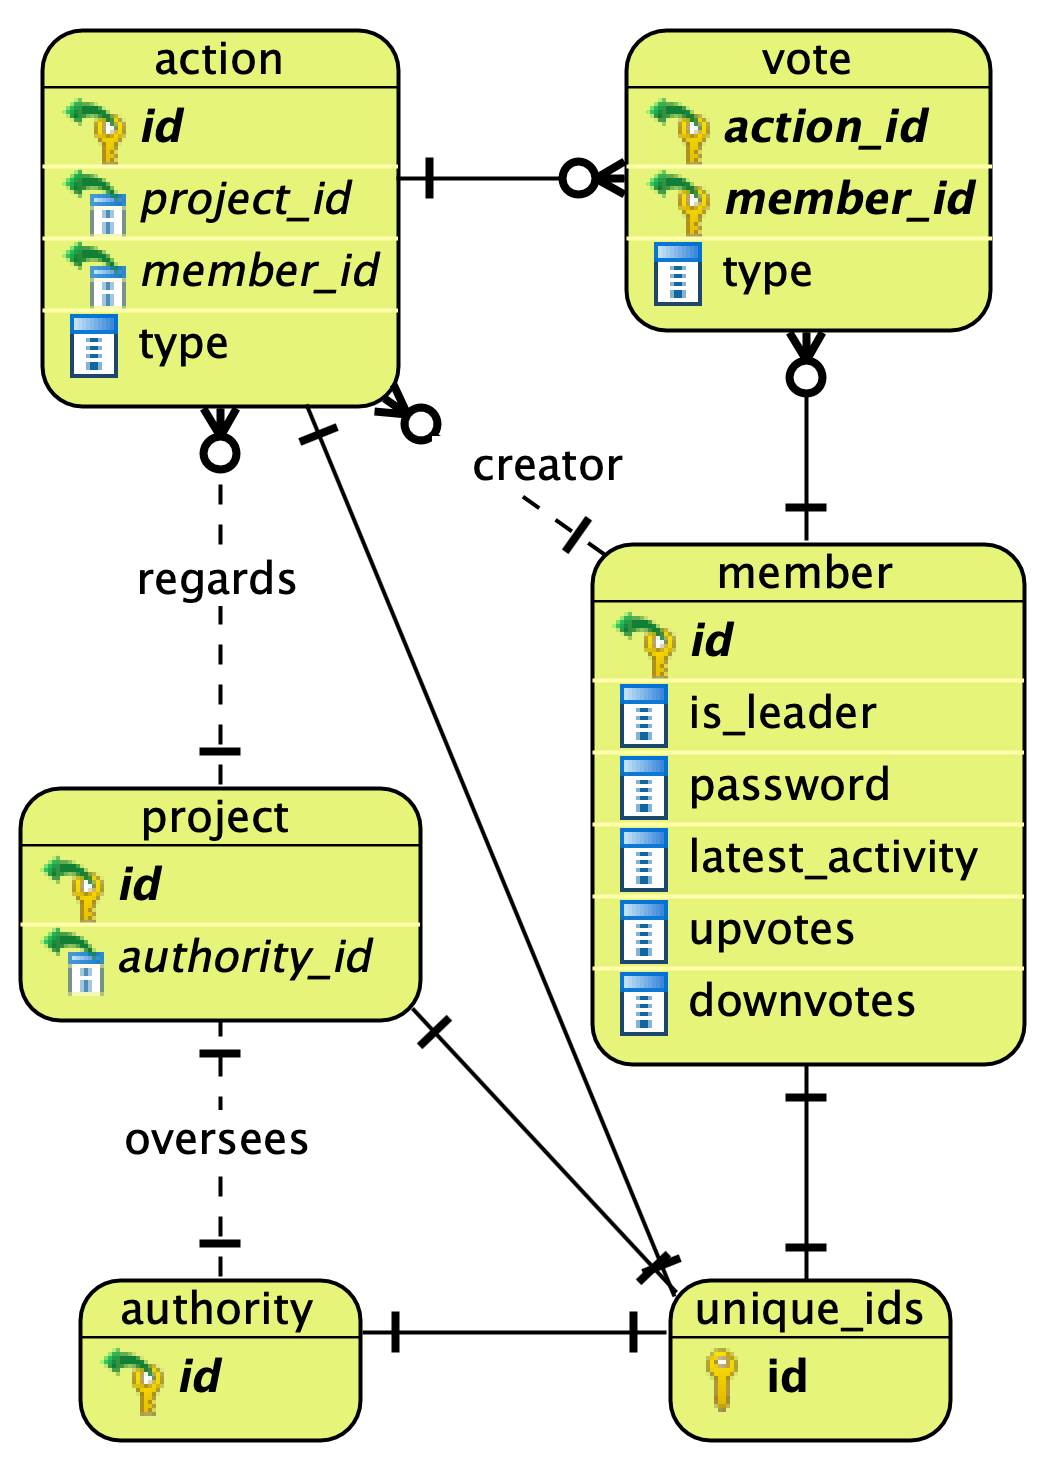
\includegraphics[scale=0.3]{ERD.png}
\end{center}

\section{Dodatkowe więzy}
\begin{itemize}
	\item Identyfikatory \texttt{member}, \texttt{action}, \texttt{project} i \texttt{authority} są globalnie unikalne.
    \item W kolumnach \texttt{upvote} oraz \texttt{downvote} w tabeli \texttt{member} znajdują się liczby głosów oddanych przez danego członka partii.
    \item W kolumnach \texttt{upvote} oraz \texttt{downvote} w tabeli \texttt{action} znajdują się sumy liczby głosów oddanych na daną akcję przez wszystkich członków partii.
\end{itemize}

\section{Uprawnienia użytkowników}
    \subsection{init}
        Ma pełne uprawnienia.
    \subsection{app}
        Może odwoływać się do zdefiniowanych funkcji.

\section{Implementacja API}
    \subsection{open}
        Otwiera połączenie z bazą danych.
    \subsection{leader}
        
    \subsection{support}
    \subsection{protest}
    \subsection{upvote}
    \subsection{downvote}
    \subsection{actions}
    \subsection{projects}
    \subsection{votes}
    \subsection{trolls}
    
\end{document}
